\documentclass[11pt]{article}		% Sets font size and document type
\usepackage{fontspec}				% Allows us to use custom fonts
\usepackage{graphicx}				% Does pictures
\usepackage{parskip}				% Removes paragraph indents
\usepackage{multicol}				% Allows for multiple columns
\usepackage{titlesec}				% Changes section title appearance
\usepackage{setspace}				% Allows you to set line spacing
\usepackage{amsmath}				% Maths typesetting
\usepackage[margin=20 mm]{geometry}	% Sets page margin
\usepackage[colorlinks=true,linkcolor=blue,citecolor=blue,urlcolor=blue]{hyperref}	
									% Allows for hypertext for references (links) - edited to hake links look like normal text rather than having a border
\doublespacing						% Double spaces - this annoys me but is unavoidable I think

%Add any more packages needed here:
\usepackage[justification=centering,font=small]{caption}	
									% Centres captions and makes them smaller
\usepackage[none]{hyphenat}			% Lines end cleanly - no hyphenation mid word
\usepackage{fancyhdr}				% Nicer headers/footers

% There is some scope for changing the paragraph spacing and spacing around section headers if you are short of space

\graphicspath{{Images/}}	% Images are in a folder called 'Images'

% Code which should allow us to attribute sections to each author - will then show the current author (mostly) at the start and end of the page
%\usepackage{etex}
%
%\newmarks\writtenBy
%
%\newcommand{\by}[1]
%{
%	\marks\writtenBy{#1}
%}
%
%\pagestyle{fancy}
%\renewcommand{\headrulewidth}{0pt}
%\renewcommand{\footrulewidth}{0pt}
%\fancyhead{}
%\fancyhead[R]{\topmarks\writtenBy}
%\fancyfoot[R]{\botmarks\writtenBy}

% Set a variable for image height, so all images are the same size and easy to change
\newlength{\imageheight}	 % Creates the variable
\setlength{\imageheight}{0.3\textwidth}  % Sets the variable

% Use Arial
\setmainfont[
BoldFont=Arial Bold.ttf,
ItalicFont=Arial Italic.ttf,
BoldItalicFont=Arial Bold Italic.ttf
]{Arial.ttf}

% Have got this working with TexStudio now - need to change compiler from default to XeLaTeX (Options > Configure TexStudio > Build > Default Compiler > XeLaTeX)
% Will be slow at first, but once the fonts have installed should work more quickly


\begin{document}
	
	\flushleft
	\raggedright

	\begin{center}
		\vspace*{2cm}
		Trinity Term 2020\\ % enter the date
		\vspace*{6cm}
		\huge{\textbf{3YP Project: Pipe Inspection Robot}}\\ 
		\vspace*{6cm}
		\large{Monty Beresford, Louis Emanuel, Joshua Gei \& Jim Laney} % Not your Bod card number
		\thispagestyle{empty} % Remove page number
	\end{center}

	\newpage
	
	\tableofcontents
	\thispagestyle{empty} % Remove page number
	\newpage

	\setcounter{page}{1}
	
	\section{Introduction}
	
	The pipe inspection robot works in underground pipes in urban areas, with a pipe diameter from 152.4 mm to 406.4 mm and with pipes at any angle, providing a map of the pipe with the location of any failures to the operator. % Needs citation for pipe sizes?
	The robot reduces the disruption caused by having to dig up large areas of pipe for inspection, since the issue can be located and smaller, less disruptive work can be undertaken.
	It is intended to provide an inspection method for pipes which cannot be inspected by the current leading method, Pipe Inspection Gauges (PIGs), which only work in horizontal or near horizontal straight pipes\textsuperscript{\cite{mills2017advances}}.
	It enters a pipe using a launch tube, and travels autonomously along the inside of the pipe, checking for evidence of cracks and corrosion and logging their location for future maintenance.
	\\
	\begin{figure}[h] % Would like to do this as a text wrapped figure but that can be finnicky so would like to agree on this as a group before attempting it
		\centering
		\includegraphics[height=\imageheight]{overviewDrawing}
		\caption{3D Sketch of robot}		% Maybe replace with 3D CAD model if possible
		\label{3DSketch}
	\end{figure}
	While inside the pipe, the robot uses three legs to maintain contact and provide the required normal force to move inside the pipe, as shown in \hyperref[3DSketch]{Figure \ref*{3DSketch}}.
	Two of these legs can be rotated to provide improved speeds over pipes at different angles, and all three legs can be extended and retracted to fit the pipe diameter the robot is currently in.
	It can navigate around bends and through pipes at different angles, without prior knowledge of the location or angle of these, and will automatically feedback to the control system in order to create an accurate map.
	\\
	The robot uses computer vision to identify cracks and corrosion, allowing it to mark where these occur for human maintenance, and then combines this with knowledge of its position to create a map of the pipe it has travelled and where issues have occurred.
	It can transmit its location using a small transmitter, which has a separate power supply so that if the robot breaks down it can be located with minimal excavation.
	
	\section{Hardware}
	
		\subsection{Locomotion}
		
			The main locomotion of the robot is a set of 3 legs with a pantograph mechanism  to allow for the adaptation to different diameters, with tracks at the end to drive the motion, as shown in \hyperref[legDesign]{Figure \ref*{legDesign}}.
			There is one leg which remains stationary at the top of the robot, and two legs which are able to rotate about the body of the robot between $10^\circ$ and $90^\circ$ to the vertical.
			At the end of each leg there is a passive joint between the leg and the track to allow for the robot to travel along surfaces which are not perpendicular to the legs, such as around bends or over uneven surfaces.
			\\
			The length of the pantograph is controlled by the force from two opposing linear actuators, which extend to a given length to set the distance of the pantograph.
			The track at the end of the pantograph is connected to a freely turning joint, which can be measured using two angular sensors to give the angle $\phi$, shown in \hyperref[legDiagram]{Figure \ref*{legDiagram}}, with the springs acting to restore $\phi$ to $0^\circ$ when under no external effects.
			In addition to this, the tracks use an active compliance joint, as shown in \hyperref[activeCompliance]{Figures \ref*{activeCompliance} \& \ref*{unevenBehaviour}}, which allows for the robot to maintain maximum surface contact at all times.
						
			\begin{figure}[h]
				\centering
				\begin{multicols}{2}
					\includegraphics[height=\imageheight]{activeCompliance}
					\caption{Function and construction of an active compliance joint. Figure from \cite{park2010normal}}
					\label{activeCompliance}
					\columnbreak
					\includegraphics[height=\imageheight]{unevenBehaviour}
					\caption{Behaviour of active compliance joint over uneven surfaces (travelling upwards). Figure from \cite{park2010normal}}
					\label{unevenBehaviour}
				\end{multicols}
			\end{figure}
		
			The ratio between the longer base links of the pantograph and then shorter tip links is 2:1, which gives the greatest range of diameters for the smallest change in the base distance\textsuperscript{\cite{okada1987mogrer}}, so we can calculate the required link length $L$ to allow the robot to adapt to the chosen range of diameters, 152.4 - 406.4 mm.
			The pantograph angles are shown in \hyperref[legDiagram]{Figure \ref*{legDiagram}}, and we can find that:
			
			\begin{align}
				r_{min} = \frac{3L}{2} \sin \left( \theta_{min} \right)
				\\
				r_{max} = \frac{3L}{2} \sin \left( \theta_{max} \right)
				\\
				\implies \Delta r = \frac{3L}{2} \left( \sin \left( \theta_{max} \right) - \sin \left( \theta_{min} \right) \right)
				\\
				L=\frac{2 \Delta r}{3 \left( \sin \left( \theta_{max} \right) - \sin \left( \theta_{min} \right) \right)}
			\end{align}
			
			If we assume that the pantograph will ideally move from an angle of $\theta_{min} = 10^\circ$ to $\theta_{max} = 60^\circ$, spanning a change in radius of 127 mm, we find that $L =$ 122.3 mm, and our smallest leg radius $r_{min} =$ 31.9 mm, not including the depth of the tracks.
			This means that our body diameter has a maximum of 88.6 mm, reduced by the track thickness, setting a constraint on the dimensions of the inner body based on our design criteria.
			
			\begin{figure}[h]
				\centering
				\begin{multicols}{2}
					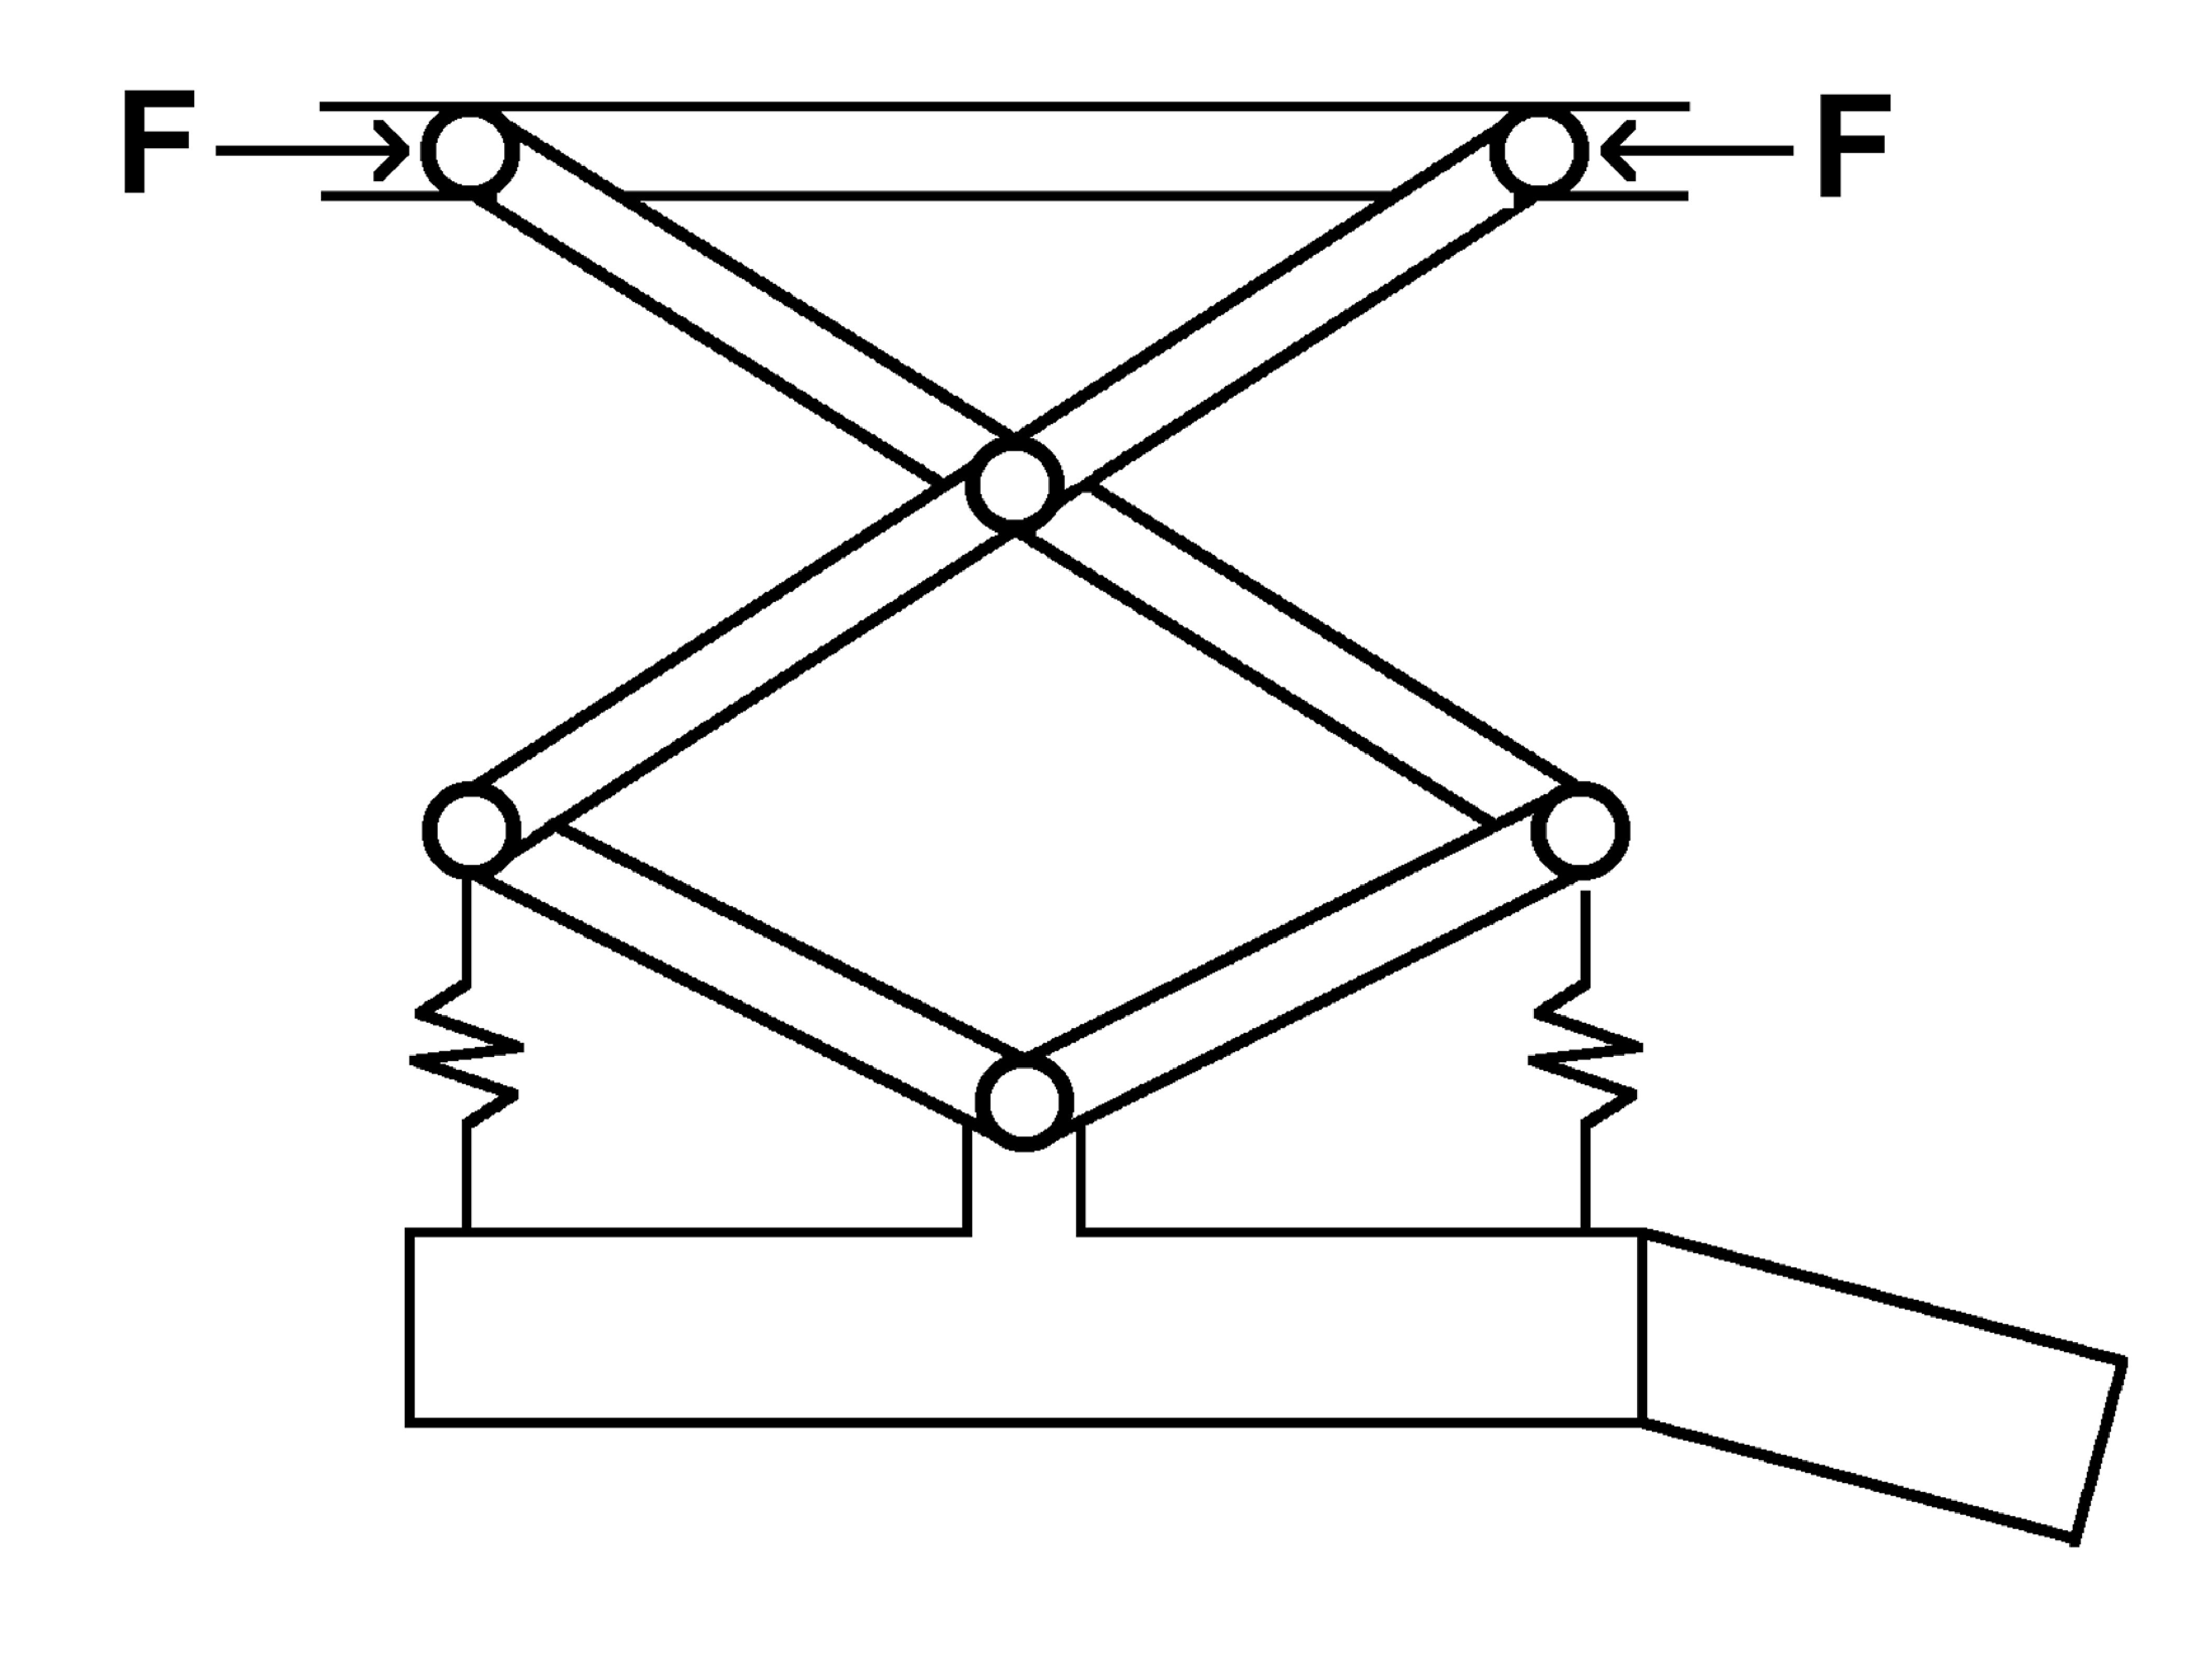
\includegraphics[height=\imageheight]{legDesign}
					\caption{Diagrammatic representation of the pantograph mechanism used for the robot's legs}
					\label{legDesign}
					\columnbreak
					
\includegraphics[height=\imageheight]{legDiagram}
					\caption{Labelled Diagram indicating angles referenced in the text}
					\label{legDiagram}
				\end{multicols}
			\end{figure}
				
		\subsection{Power}
		
		\subsection{Sensing}
		
		\subsection{Communications}
		
		\subsection{External Hardware}
	
		\subsection{Materials and Construction}
	
	\section{Software}
	
		\subsection{Actuation Control}
		
		\subsection{Bend \& Angle Detection}
		
		\subsection{Crack \& Corrosion Detection}
		
		\subsection{Mapping and Location}
		
		\subsection{Communications}
	
	\pagebreak		% Temp page break for references - might end up replacing with a multicolumn environment later
	
	% In order to make a reference to an entry in the bibliography, use \cite{}
	% TexStudio will suggest names from the bib file - not sure about overleaf but otherwise use the first entry in the string
	% Make sure bibliography is set to use BibTex rather than BibLatex
	% See mybib.bib for an example bib file format - most things should be able to give it to you in this format
	% Our actual bibliography will be 3YPbib.bib
	% Currently using google scholar default ids - should help prevent duplication of references but will need to be checked
	
	\nocite{*} 				% By default Latex will not show uncited references, uncomment this line to show all references in the bib file
	
	\begingroup\onehalfspacing
		{\small
			\bibliographystyle{ieeetr}
			\bibliography{3YPbib}
		}
	\endgroup

\end{document}
